\chapter{离障碍多远：二维距离场}
\begin{notebox}
\textbf{目标}\quad 从占据图构造距离场，推导任意位置的插值与梯度，并计算保守净空。\\
\textbf{先修}\quad 第 07、11 章的栅格、欧氏距离与碰撞几何。
\end{notebox}

\section{先看一个圆的距离场}
A* 回答“哪条路可以通行”。轨迹优化还希望知道：离障碍有多远，向哪个方向挪一点能增加间隙？
距离场给每个位置赋一个数，梯度则描述这个数增加最快的方向。
先运行一个有解析答案的圆形实验：
\begin{lstlisting}[language=bash]
ros2 run motion2d esdf_demo tmp/ch12_esdf
/usr/bin/python3 scripts/plot_ch12_esdf.py
\end{lstlisting}
半径为 1 m、圆心在原点的圆，其有符号距离为
\begin{equation}
d_{\rm circle}(x,y)=\sqrt{x^2+y^2}-1.
\end{equation}
圆外正、圆内负、边界零。例如 $(1.3,0)$ 距圆边 $.3$ m，$(.8,0)$ 距圆边向内 $.2$ m。
对平方根用链式法则，在 $(x,y)\neq(0,0)$ 处有
\begin{equation}
\frac{\partial d}{\partial x}=\frac{2x}{2\sqrt{x^2+y^2}},\qquad
\frac{\partial d}{\partial y}=\frac{2y}{2\sqrt{x^2+y^2}},\qquad
\nabla d=\frac{(x,y)^\top}{\sqrt{x^2+y^2}}.
\end{equation}
梯度朝圆外，长度为 1；移动小位移 $\Delta p$，距离变化约为 $\nabla d^\top\Delta p$。
圆心处所有径向方向都等价，而且沿 $x$ 轴的距离为 $|x|-1$，左右导数分别为 $-1,+1$，
所以那里没有唯一梯度。实验把这个圆离散成占据格，再研究离散场与解析圆之间的差别。

\section{格子中心距离与方格净空}
输入使用未膨胀的观测栅格。沿用上一章的标签策略：已观测且编码不超过 35 才自由，
未知默认阻塞；外围补一圈阻塞格，使靠近地图边界的位置也能感知外部空间。
记阻塞格中心集合为 $O_c$、自由格中心集合为 $F_c$，定义
\begin{equation}
d_i=\begin{cases}
\min_{c_j\in O_c}\|c_i-c_j\|,&i\text{ 自由},\\
-\min_{c_j\in F_c}\|c_i-c_j\|,&i\text{ 阻塞}.
\end{cases}
\end{equation}
自由位置寻找最近阻塞中心，阻塞位置寻找最近自由中心后加负号。
这样两侧的数值沿着“离开障碍”的方向增加，适合为优化提供移动方向。

中心之间的距离还包含方格本身的半个宽度。例如墙面位于 $x=0$，
紧邻墙面的阻塞中心位于 $-\rho/2$，自由中心位于 $+\rho/2$。
自由中心到墙的真实间隙为 $\rho/2$，到阻塞中心则为 $\rho$。
后面会将中心距离转换成到阻塞方格的保守下界。

\begin{center}
\begin{tikzpicture}[x=2cm,y=1cm,>=Stealth]
\fill[navy!12] (-1,-.45) rectangle (0,.45);
\draw[navy,thick] (0,-.55)--(0,.55);
\draw[->] (-1.15,0)--(1.15,0) node[right]{$x$};
\fill[navy] (-.5,0) circle(2pt);
\fill[tealblue] (.5,0) circle(2pt);
\node[below] at (-.5,-.2) {阻塞中心};
\node[below] at (.5,-.2) {自由中心};
\draw[<->] (-.5,.95)--(.5,.95) node[midway,above]{中心距 $\rho$};
\draw[<->] (0,1.7)--(.5,1.7) node[midway,above]{净空 $\rho/2$};
\draw[dotted] (-.5,.1)--(-.5,.85);
\draw[dotted] (.5,.1)--(.5,1.6);
\draw[dotted] (0,.6)--(0,1.6);
\end{tikzpicture}
\end{center}
整张地图阻塞时，自由中心集合为空，无法得到有限的内部距离；
代码用 $-\infty$ 标记，并让连续查询返回空结果。
整张地图自由时，外围阻塞圈仍提供种子，因此距离由外部边界决定。

\section{把二维最近距离拆成两次一维计算}
直接对每个格子枚举所有障碍中心，计算量会随格数和障碍数相乘增长。
欧氏距离变换（EDT）利用平方距离的结构来减少搜索。
先以格子索引为坐标，将种子格的代价设为 0，其余格设为 $+\infty$：
\begin{equation}
f(i,j)=\begin{cases}0,&(i,j)\text{ 是种子},\\+\infty,&\text{其他格}.
\end{cases}
\end{equation}
于是每个位置到最近种子的平方距离为
\begin{equation}
D(x,y)=\min_{i,j}\big[(x-i)^2+(y-j)^2+f(i,j)\big].
\end{equation}
这里的 $x,y,i,j$ 都是整数索引。非种子位置的无穷代价使它不会成为最小值。
对固定的 $i$，$(x-i)^2$ 与 $j$ 无关，可以提出内部最小值：
\begin{align}
A(i,y)&=\min_j[(y-j)^2+f(i,j)],\\
D(x,y)&=\min_i[(x-i)^2+A(i,y)].
\end{align}
第一式逐列计算上下距离，第二式逐行比较不同列的候选。
这是对所有候选做同一次最小化，只是改变了枚举顺序，结果保持一致。

例如种子在 $(0,0)$ 与 $(2,1)$，查询 $(1,2)$。
处理列后，第 2 行在列 $0,1,2$ 的值分别为 $4,+\infty,1$。
再加横向距离平方：$1+4,0+\infty,1+1$，最小值为 2，
对应种子 $(2,1)$。若 $\rho=.1$ m，则米制距离为 $.1\sqrt2$ m。
一般地，索引平方距离转为米制距离需要
\begin{equation}d=\rho\sqrt D.\end{equation}
以阻塞中心为种子做一次 EDT，以自由中心为种子再做一次，随后按原标签选择正负值。

\code{squaredDistanceTransform} 中的列循环与行循环正好对应 $A$ 和 $D$。

\section{一维距离变换：维护抛物线的最低部分}
\subsection{由平方距离得到抛物线交点}
两次一维处理都具有相同形式：给定数组 $f(q)$，求
\begin{equation}D(x)=\min_q[f(q)+(x-q)^2].\end{equation}
将每个有限的 $f(q)$ 画成曲线 $P_q(x)=f(q)+(x-q)^2$。
它是一条开口相同、顶点为 $(q,f(q))$ 的抛物线。
对每个 $x$ 取最低的一条，得到的曲线称为\textbf{下包络}。
列处理后的 $f(q)$ 可能是非零平方距离，因此需要这种一般形式。

按 $q$ 从小到大加入新曲线。设已经保留的末条曲线中心为 $v<q$，两条曲线相等时
\begin{align}
f(q)+x^2-2qx+q^2&=f(v)+x^2-2vx+v^2,\\
2(q-v)x&=f(q)+q^2-f(v)-v^2.
\end{align}
共同的 $x^2$ 消掉了，所以交点只有一个：
\begin{equation}s=\frac{f(q)+q^2-f(v)-v^2}{2(q-v)}.\end{equation}
两曲线之差为 $P_q(x)-P_v(x)=2(q-v)(s-x)$。
因为 $q-v>0$，$x<s$ 时新曲线较高，$x>s$ 时新曲线较低。
因此新加入的中心只会从某个分界点开始，在右边接替旧曲线。

\subsection{一次删除中间曲线的手算}
令 $f(0)=0,f(1)=4,f(2)=0$，有
$P_0=x^2$、$P_1=4+(x-1)^2$、$P_2=(x-2)^2$。
开始只保留 $P_0$。加入 $P_1$ 时，交点为 $(4+1)/2=2.5$，暂记它从 2.5 开始胜出。
加入 $P_2$ 时，它与 $P_1$ 的交点为 $(4-5)/2=-.5$，早于 $P_1$ 原来的胜出位置 2.5。
也就是说，$P_1$ 还没来得及低于 $P_0$，就已被 $P_2$ 压在上方，因此可删除。
随后比较 $P_2$ 与 $P_0$，交点为 $4/4=1$。
最终 $x\leq1$ 选 $P_0$，$x\geq1$ 选 $P_2$；在交点两者数值相同。

\begin{center}
\begin{tikzpicture}
\begin{axis}[width=.8\linewidth,height=5.2cm,xmin=-.4,xmax=2.4,ymin=0,ymax=6.1,
  xlabel={查询索引 $x$},ylabel={平方代价},grid=major,
  legend style={at={(.5,1.05)},anchor=south,legend columns=2,font=\small},
  tick label style={font=\small}]
\addplot[navy,domain=-.4:2.4,samples=80]{x^2};\addlegendentry{$P_0=x^2$}
\addplot[orange!85!black,dashed,domain=-.4:2.4,samples=80]{4+(x-1)^2};\addlegendentry{$P_1=4+(x-1)^2$}
\addplot[tealblue,domain=-.4:2.4,samples=80]{(x-2)^2};\addlegendentry{$P_2=(x-2)^2$}
\addplot[black,very thick,domain=-.4:1,samples=35]{x^2};\addlegendentry{下包络}
\addplot[black,very thick,domain=1:2.4,samples=35,forget plot]{(x-2)^2};
\addplot[muted,dotted,forget plot] coordinates{(1,0)(1,1)};
\end{axis}
\end{tikzpicture}
\end{center}

\subsection{数组如何保存这条下包络}
\code{sites} 保存仍可能最低的中心索引，\code{begin} 保存每条曲线开始胜出的横坐标。
第一条曲线从 $-\infty$ 开始。加入新中心时，若交点不晚于末条曲线的 \code{begin}，
就删除末条并继续向前比较；否则将新曲线和分界点放在末尾。

\par\noindent\begin{minipage}{\linewidth}
\lstinputlisting[language=C++,linerange={edt_envelope_begin-edt_envelope_end},
  includerangemarker=false]{../ros2_ws/src/motion2d/src/mapping/distance_transform.cpp}
\end{minipage}\par
\code{last} 指向有效数组的末端；\code{--last} 删除一个候选，
随后 \code{++last} 腾出新位置。无穷的输入在进入这个循环前跳过，因为它们永远不会取得有限最小值。
包络建好后，查询 $x=0,1,\ldots$，用一个只向右移动的指针找到对应曲线即可。

每个中心最多入栈一次、出栈一次，读取阶段的指针也只向右经过每个中心一次。
因此长度为 $n$ 的一维数组只需与 $n$ 成正比的工作量，写为 $O(n)$。
宽 $W$、高 $H$ 的地图，列处理为 $W$ 次 $O(H)$，行处理为 $H$ 次 $O(W)$，合计为 $O(WH)$。
这套方法由 Felzenszwalb 与 Huttenlocher 系统给出。\footnote{原始论文：
\href{https://theoryofcomputing.org/articles/v008a019/}{Distance Transforms of Sampled Functions}，2012，第2节。}
用上面的三条抛物线逐步填写 \code{sites} 和 \code{begin}，就能追踪循环中的删除与追加。

\section{从四个中心值插出任意位置的距离}
\subsection{从一维线性插值到双线性插值}
距离数组存的是格子中心样本。若左下中心的索引为 $(i,j)$，其米制坐标是
$(o_x+(i+\tfrac12)\rho,o_y+(j+\tfrac12)\rho)$。
因此查询点先换成中心索引坐标：
\begin{equation}
\xi=\frac{x-o_x}{\rho}-\frac12,\qquad\eta=\frac{y-o_y}{\rho}-\frac12.
\end{equation}
取 $i=\lfloor\xi\rfloor,j=\lfloor\eta\rfloor$，
$u=\xi-i,v=\eta-j$ 表示在四个中心围成的方块内横、纵方向走过的比例，均在 $[0,1]$ 内。
查询范围限定在最外围中心组成的闭矩形；位于最大索引处时，用最后一个插值块并取比例 1。

\begin{center}
\begin{tikzpicture}[x=2.2cm,y=2.2cm,>=Stealth]
\draw[tealblue] (0,0) rectangle (1,1);
\foreach \x/\y/\label in {0/0/00,1/0/10,0/1/01,1/1/11} {
 \fill[navy] (\x,\y) circle(2pt);
}
\node[below left] at (0,0) {$d_{00}$};\node[below right] at (1,0) {$d_{10}$};
\node[above left] at (0,1) {$d_{01}$};\node[above right] at (1,1) {$d_{11}$};
\draw[dashed] (.3,0)--(.3,1);\draw[dashed] (0,.7)--(1,.7);
\fill[tealblue] (.3,.7) circle(2pt);\node[above right] at (.3,.7) {$p$};
\draw[<->] (0,-.32)--(.3,-.32) node[midway,below] {$u\rho$};
\draw[<->] (1.4,0)--(1.4,.7) node[midway,right] {$v\rho$};
\end{tikzpicture}
\end{center}
在一条线上，端点值为 $a,b$，满足两端值的直线是 $a+u(b-a)=(1-u)a+ub$。
所以先沿上下两行插值，再沿纵向插值：
\begin{align}
d_{\rm bottom}&=(1-u)d_{00}+ud_{10},\quad
 d_{\rm top}=(1-u)d_{01}+ud_{11},\\
\widetilde d&=(1-v)d_{\rm bottom}+v d_{\rm top}\\
&=(1-u)(1-v)d_{00}+u(1-v)d_{10}+(1-u)vd_{01}+uvd_{11}.
\end{align}
四个权重均非负，并且和为
$(1-v)[(1-u)+u]+v[(1-u)+u]=1$，所以插值值处于四个样本值的最小值与最大值之间。

\subsection{对权重求导，再换回米制坐标}
固定样本值，对 $u$ 求导，上下两行分别产生差值 $d_{10}-d_{00}$ 和 $d_{11}-d_{01}$；
对 $v$ 求导则得到上行值减下行值。
利用 $du/dx=dv/dy=1/\rho$，得到
\begin{align}
\frac{\partial\widetilde d}{\partial x}
&=\frac{(1-v)(d_{10}-d_{00})+v(d_{11}-d_{01})}{\rho},\\
\frac{\partial\widetilde d}{\partial y}
&=\frac{(1-u)(d_{01}-d_{00})+u(d_{11}-d_{10})}{\rho}.
\end{align}
距离单位为 m，坐标单位也为 m，因此梯度分量的单位为 m/m。
少除一次 $\rho$，就会把“走过一个格子时变化多少”误当成“走过一米时变化多少”。

\par\noindent\begin{minipage}{\linewidth}
\lstinputlisting[language=C++,linerange={esdf_bilinear_begin-esdf_bilinear_end},
  includerangemarker=false]{../ros2_ws/src/motion2d/src/mapping/esdf.cpp}
\end{minipage}\par
手算一个带交叉项的例子：以左下中心为局部原点，将米制坐标数值代入
$f(x,y)=2x+3y+xy$，取边长 $\rho=.2$。
四角值为 $0,.4,.6,1.04$；在 $u=.3,v=.7$ 处，局部坐标为 $(.06,.14)$，
插值值为 $.5484$，梯度为 $(2.14,3.06)$，与直接求导 $(2+y,3+x)$ 一致。
这也是 \textbf{代码练习 ch12-1} 的核对例子。

\subsection{怎样理解梯度的变化}
每个插值块内部可以直接使用上述导数；换到相邻块后，样本差值改变，梯度可能跳变。
在前面的直墙例子中，阻塞中心取 $-\rho$、自由中心取 $+\rho$，二者仅相距 $\rho$，
所以两中心之间插值的斜率为 $(\rho-(-\rho))/\rho=2$。
这说明本章的中心距离插值场可以提供平滑块内的移动方向，梯度长度则由离散样本决定。
代码原样保留这个导数，便于后面计算轨迹代价的链式梯度。

\section{从插值距离推导保守净空}
原始插值可能因样本间距和方格面积高估净空。
下面只用三角不等式，推导一个始终不大于地图实际间隙的数。
设四个插值中心都自由，记它们为 $c_k$，非负权重为 $w_k$，且 $\sum_k w_k=1$。

\subsection{移动一段距离，最近中心距离最多变化多少}
记 $d_c(p)$ 为查询点到最近阻塞中心的无符号距离。
假设 $c_*$ 是离 $q$ 最近的阻塞中心，那么
\begin{equation}
d_c(p)\leq\|p-c_*\|\leq\|p-q\|+\|q-c_*\|
=\|p-q\|+d_c(q).
\end{equation}
第一步是在所有中心中取最小值，第二步是三角不等式。
交换 $p,q$ 再写一次，就得到
\begin{equation}|d_c(p)-d_c(q)|\leq\|p-q\|.\end{equation}
这个性质称为 1-Lipschitz，直观上就是移动一米，最近距离至多改变一米。
特别地，每个中心样本给出下界 $d_c(p)\geq d_c(c_k)-\|p-c_k\|$。
乘以 $w_k$ 再相加，左边因权重和为 1 仍是 $d_c(p)$，于是
\begin{equation}
d_c(p)\geq\underbrace{\sum_k w_kd_c(c_k)}_{\widetilde d(p)}
-\underbrace{\sum_k w_k\|p-c_k\|}_{E(p)}.
\end{equation}
$E$ 是从四个中心插值到查询点时，为可能高估的距离预留的修正量。

\subsection{再把中心换成有面积的方格}
障碍格内任一点 $z$ 到格子中心 $c$ 的距离至多为半对角线
$h=\sqrt{(\rho/2)^2+(\rho/2)^2}=\rho/\sqrt2$。
又由三角不等式的变形，
\begin{equation}
\|p-z\|\geq\|p-c\|-\|z-c\|\geq d_c(p)-h.
\end{equation}
对所有阻塞方格中的 $z$ 取最小值，这个下界仍成立。
最近的地图外部点位于边界，外围阻塞圈的方格覆盖该边界，因此同一推导也包括地图外部。
将两个修正合在一起，并利用几何间隙非负，得到
\begin{equation}
\underline d(p)=\max\left(0,\widetilde d(p)-\sum_{k=1}^4 w_k\|p-c_k\|-\frac{\rho}{\sqrt2}\right).
\end{equation}
这对应 \code{EsdfSample::clearance_lower_bound}。
\code{sample} 先检查四个中心标签，再用四个双线性权重累加 \code{error}，
最后减去 \code{resolution/std::sqrt(2.)}。
若四个中心中包含阻塞格，采用零下界；零值表示当前计算还未给出正间隙，可继续用精确几何检查。

例如 $\rho=.2$ m，四角中心距离为 $(.6,.8,.6,.8)$ m，查询插值块中心。
四个权重都是 $1/4$，$\widetilde d=.7$ m，各角距离为 $.2/\sqrt2$ m，故
\begin{equation}
E=\frac{.2}{\sqrt2},\qquad
\underline d=.7-2\frac{.2}{\sqrt2}\approx.4172\ \text{m}.
\end{equation}
机器人半径 $.2$ m、裕量 $.05$ m 时，$.4172>.25$，这个中心位置满足间隙要求。
这里的下界针对当前占据方格所表达的几何；新观测修改地图后，需要相应重算距离场。

\subsection{三个返回值各自怎样使用}
\begin{center}\small
\begin{tabular}{lll}\toprule
字段 & 计算意义 & 后续用途\\\midrule
\code{distance} & 有符号中心距离的插值 & 构造避障代价\\
\code{gradient} & 上一项对 $x,y$ 的偏导 & 反传轨迹梯度\\
\code{clearance_lower_bound} & 到阻塞方格及外部的净空下界 & 检查圆心间隙\\\bottomrule
\end{tabular}
\end{center}
半径在这里通过 $\underline d>r+m$ 处理；输入用未膨胀地图，
而第十一章的配置空间地图已把半径计入，按中心点检查即可。
\code{gradient} 对应插值距离，计算下界时还额外减去了随位置变化的 $E$，所以两者导数不同。

对一条轨迹，检查一个位置只能确定这一处的间隙。
即使两个端点都有正距离，它们之间也可能穿过障碍。
第十三章将用安全凸区域包住一段路径，第十六章再利用曲线的控制点性质检查整段包含关系。

\section{用可以手算的场核对实现}
\begin{enumerate}
\item 从单个种子开始，枚举少量格子的距离平方，与两次一维 EDT 的中间数组逐项比较。
再试三条抛物线的删除例子，观察候选数组怎样缩短。
\item 给四角指定常数或双线性函数值，代入解析梯度，并用中心差分
$[d(p+\epsilon e_i)-d(p-\epsilon e_i)]/(2\epsilon)$ 核对。选取扰动前后都在同一插值块内的点。
\item 对几个轴对齐阻塞方格，用第七章的点到方格距离算出精确净空，
与 $\underline d$ 比较，并解释插值修正和半对角线修正各减掉了什么。
\end{enumerate}
这三组练习依次核对离散最小值、连续插值和面积修正，帮助区分不同来源的误差。

\section{分辨率实验与练习}
\begin{figure}[h]
\centering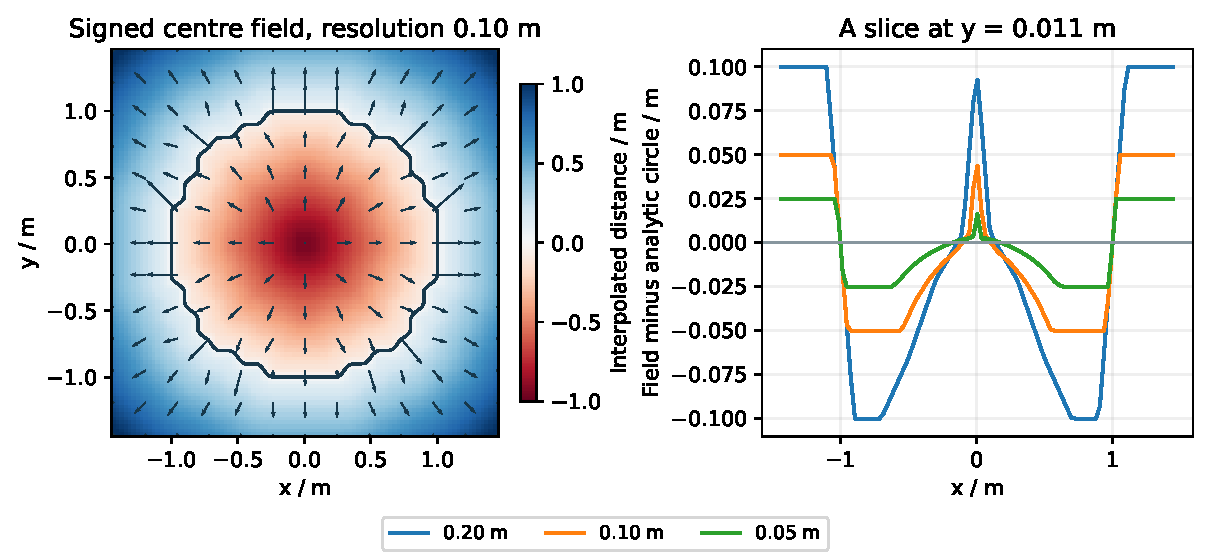
\includegraphics[width=.84\linewidth]{figures/ch12_esdf.pdf}
\caption{左：0.1 m 格的有符号场与插值梯度，坐标等比例。右：固定 y 的距离误差切片。
不同分辨率都存在栅格化和中心距离误差，靠近界面时插值也影响结果。}
\end{figure}
\begin{center}\small
\pgfplotstabletypeset[col sep=comma,
columns={resolution,cells,mae_m,max_error_m,median_us,p95_us},
columns/resolution/.style={column name=$\rho$/m,fixed,precision=2},columns/cells/.style={column name=格数},
columns/mae_m/.style={column name=平均误差/m,fixed,precision=4},
columns/max_error_m/.style={column name=最大误差/m,fixed,precision=4},
columns/median_us/.style={column name=中位数/$\mu$s,fixed,precision=1},
columns/p95_us/.style={column name=P95/$\mu$s,fixed,precision=1},
every head row/.style={before row=\toprule,after row=\midrule},
every last row/.style={after row=\bottomrule}]{data/ch12_esdf.csv}
\end{center}
给定地图为 $8\times8$ m；中心位于半径 1 m 圆内的格子标为占据。
三组都使用同一查询晶格，统计 $0.3\leq\|p\|\leq1.6$ m 环带内与解析圆距离的绝对误差。
这是栅格对圆的近似实验：一部分误差来自圆被方格表示，另一部分来自中心距离及插值。两种几何的边界位置也会随分辨率变化。
每个分辨率预热 5 次，计时 100 次，含分类、补边界和两个 EDT，不含 ROS 序列化。
表中更细网格的平均误差更小，构建时间更长。
分辨率减半时，每边格数约翻倍，二维总格数约变为四倍，正好可用来观察 $O(WH)$ 的规模变化。
每次保留相同查询点，误差才是在相同空间位置上比较。
单个位置可能因圆边落在不同格子内而出现误差波动。
平均绝对误差为 $N^{-1}\sum_i|\widetilde d(p_i)-d_{\rm circle}(p_i)|$，
最大误差则取这些绝对值中的最大者。100 次耗时排序后，表中的中位数取第 51 个，P95 取第 95 个，
分别反映一次典型运行和较慢运行的耗时。

\textbf{练习 ch12-1：}补全 bilinearGradient。给定
$f(x,y)=2x+3y+xy$ 在 $0,\rho$ 四角的值，验证 $\rho=0.2$ m、$u=0.3,v=0.7$ 时
梯度为 $(2.14,3.06)$。再验证常数场梯度为零。
推导题与代码提示见 \path{exercises/ch12}。

\textbf{理解与实验：}画解析圆场；解释圆心处不可微、中心距与边界距的差别。
改变分辨率，报告误差、格数和构建时间，保留相同查询点与计时范围。
常见错误是忘记开方、忘记乘分辨率、把索引坐标当米数，以及使用已经膨胀的地图再扣半径。
下面将距离场接入 ROS 可视化。

\section{ROS 距离通道与梯度显示}
\begin{lstlisting}[language=bash]
ros2 launch motion2d_bringup ch12.launch.py
ros2 topic echo /esdf/status
# In a separate terminal, with the same ROS_DOMAIN_ID:
/usr/bin/python3 scripts/check_ch12.py
/usr/bin/python3 scripts/plot_ch12_observed.py
\end{lstlisting}
esdf\_node 只订阅 /map，每张观测地图独立构建一个距离场。
本章启动沿用上一章的真值定位和激光观测建图；距离场的全部几何输入来自 /map。
输入与 A* 共用同一套自由阈值、未知策略和轴对齐地图验证，避免两者解释不同的地图。

\begin{center}\small
\begin{tabular}{lll}\toprule
话题 & 类型 & 语义 \\\midrule
/esdf/cloud & PointCloud2 & x、y、z、distance 四个 FLOAT32 \\
/esdf/gradients & MarkerArray & map 中的梯度方向箭头 \\
/esdf/status & String & ready / no\_finite\_field / invalid\_map \\\bottomrule
\end{tabular}
\end{center}
点云保持原地图的 width、height，按 $i=yW+x$ 行主序存储；每点 16 字节，
行步长为 $16W$。x、y 是格子中心的米制坐标，z 固定为零。
\textbf{distance 字段存有符号中心距离，单位 m}；z 用于点的位置高度，固定为零以便在平面上显示。
全阻塞时保留 $-\infty$ 并设置 is\_dense=false，同时发布 no\_finite\_field 和空箭头。
地图格式错误时清空点云与标记，不保留上一次的有效显示。

RViz 的 Color Transformer 选择 Intensity，Channel Name 选择 distance。
预设用 $[-0.5,2.0]$ m 固定颜色范围，超出范围只在显示颜色上饱和，消息里的数值不变。
Size (m) 默认匹配 0.1 m 分辨率；修改地图分辨率后应相应调整显示方块大小。
配置空间掩码、观测图与 ESDF 是不同产物，可在 Displays 中切换比较。

梯度默认每隔 10 格显示一个箭头，箭头方向朝距离增加处。
显示长度为 $\min(0.4,0.2\|\nabla\widetilde d\|)$ m，箭头头部随短箭头缩放；
例如梯度模长为 1 时画 $.2$ m 箭头，模长为 3 时按上限画 $.4$ m，便于在同一画面内比较方向。
\lstinputlisting[language=C++,linerange={esdf_arrow_begin-esdf_arrow_end},
  includerangemarker=false]{../ros2_ws/src/motion2d/src/nodes/esdf_node.cpp}
消息沿用地图时间戳与 map 系，QoS 保留最新场。时间回退后直接用新地图重建；
晚加入的 RViz 读取当前快照。

\clearpage
\section{读一次真实距离消息}
下图来自实际 ROS 的距离点云与箭头消息，固定为 reset 后 100 步、0.5 s。
图仅截取默认随机世界左下部分；负值同时包含占据、不确定和按策略阻塞的未知区域。
颜色不能代替原始占据图中的观测来源信息。

\begin{figure}[!ht]
\centering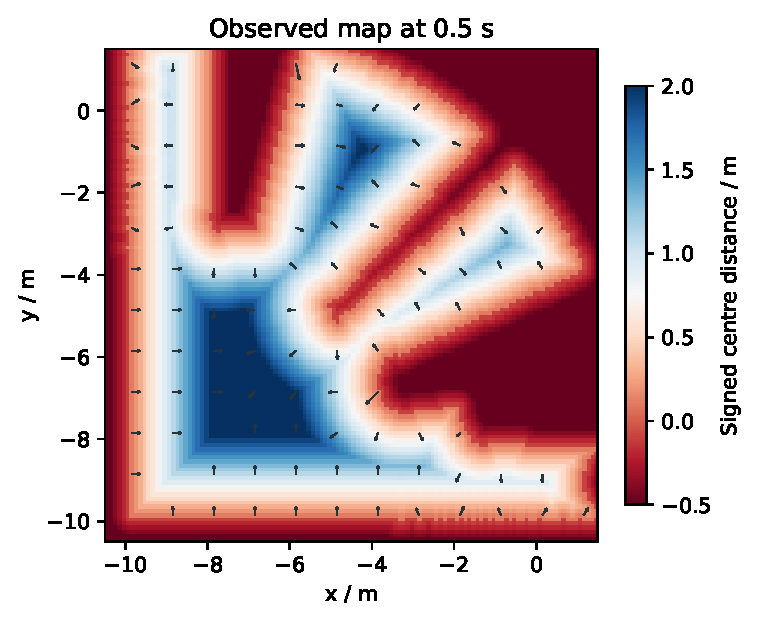
\includegraphics[width=.72\linewidth]{figures/ch12_observed.pdf}
\caption{实际观测距离场与消息中的梯度箭头。坐标为米且等比例，颜色在固定范围内显示。
图中箭头采用消息给定的位置与方向。}
\end{figure}

从地图中任选一个自由格，枚举所有阻塞中心及外围种子，手算其最近中心距离，
再读取点云同一索引的 \code{distance} 字段比较。
例如宽度为 220、索引 $(x,y)=(3,2)$，其点编号为 $2\times220+3=443$，
点起始字节为 $443\times16=7088$，distance 位于该点的第 12 字节偏移，因此从 7100 字节开始读取。
三个位置字段和一个距离字段均为四字节浮点数，所以每点合计 16 字节。

再分别输入全未知图与全自由图：全未知图缺少自由中心，显示不可用场；
全自由图仍可看到朝地图内部增大的正距离，因为外部补了一圈阻塞格。
将未知策略和颜色范围放在一起观察，可以理解同一颜色背后可能对应不同观测状态。

\textbf{消息练习：}
\begin{enumerate}
\item 从 /esdf/cloud 读取一格的四个字段，手算中心坐标和行字节偏移。
\item 把 esdf.gradient\_stride 从 10 改为 5，比较箭头密度，说明为何数值距离不变。
\item 对全自由小地图，解释为什么越靠近地图边界，正距离越小。
\end{enumerate}
独立检查入口、命令和评分见本章练习说明。
